\documentclass[tikz,border=2pt]{standalone}
\usepackage{amsmath}
\usepackage{pgfplots}
\pgfplotsset{compat=1.18}

\begin{document}
% Weierstrass M-test: each f_n lives inside a band of half-width M_n = ||f_n||_oo, and the band
% widths add up to a finite number, so the series of functions converges uniformly.
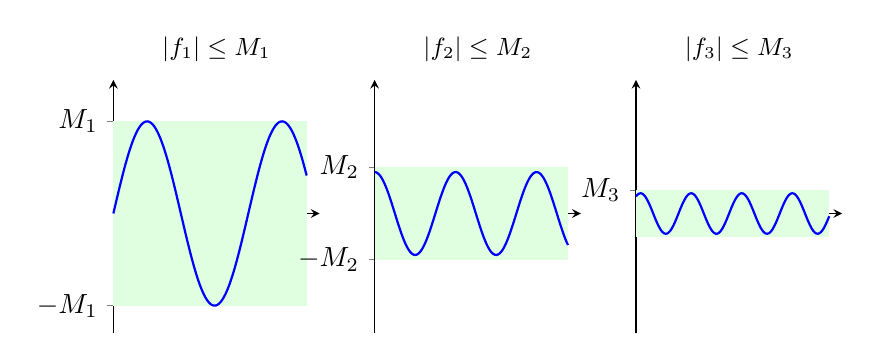
\begin{tikzpicture}
	\begin{axis}[
		name=a1,
		axis lines=middle, xmin=0, xmax=3.2, ymin=-1.3, ymax=1.45,
		xtick=\empty, ytick={1,-1}, yticklabels={$M_1$,$-M_1$},
		width=4.2cm, height=4.8cm, clip=false, samples=120, smooth,
		title={$|f_1|\le M_1$}, title style={font=\small, yshift=-3pt}
		]
		\fill[green!12] (axis cs:0,-1) rectangle (axis cs:3,1);
		\addplot[blue, thick, domain=0:3] {sin(deg(3*x))};
	\end{axis}
	\begin{axis}[
		name=a2, at={(a1.east)}, anchor=west, xshift=0.7cm,
		axis lines=middle, xmin=0, xmax=3.2, ymin=-1.3, ymax=1.45,
		xtick=\empty, ytick={0.5,-0.5}, yticklabels={$M_2$,$-M_2$},
		width=4.2cm, height=4.8cm, clip=false, samples=120, smooth,
		title={$|f_2|\le M_2$}, title style={font=\small, yshift=-3pt}
		]
		\fill[green!12] (axis cs:0,-0.5) rectangle (axis cs:3,0.5);
		\addplot[blue, thick, domain=0:3] {0.45*cos(deg(5*x))};
	\end{axis}
	\begin{axis}[
		name=a3, at={(a2.east)}, anchor=west, xshift=0.7cm,
		axis lines=middle, xmin=0, xmax=3.2, ymin=-1.3, ymax=1.45,
		xtick=\empty, ytick={0.25}, yticklabels={$M_3$},
		width=4.2cm, height=4.8cm, clip=false, samples=120, smooth,
		title={$|f_3|\le M_3$}, title style={font=\small, yshift=-3pt}
		]
		\fill[green!12] (axis cs:0,-0.25) rectangle (axis cs:3,0.25);
		\addplot[blue, thick, domain=0:3] {0.22*sin(deg(8*x+1))};
	\end{axis}
\end{tikzpicture}
\end{document}
